\chapter{模板的基础使用说明}

\section{模板基本说明}
使用本模板,您应首先具备基本的\LaTeX 知识,如果您刚刚接触\LaTeX,建议您先学习相关的用户文档或教程。

模板文件名为ustcthesis.cls。方便起见,将该文件放置在与论文主文件同一文件夹中即可。如果需要使用增强功能,模板提供了一个名为ustcxtra.cls的补充包。将该文件放置在与论文主文件同一文件夹中即可。

模板提供一个文档类ustcthesis,使用\verb|\documentclass{ustcthesis}|来加载模板。

模板可以使用ctexbook文档类的相应选项,默认加载的是 cs4size, a4paper, fancyhdr, fntef。需要注意的是默认加载 \emph{双面/章节从奇数页开始} 选项,如果需要\emph{单面} 选项,请使用:
\begin{Code}
\documentclass[<学位>,oneside,openany]{ustcthesis}
\end{Code}

\begin{table}[htp]
\centering
\tabcaption{模板提供的新文档选项}
\label{tab:newdocopt}
\begin{tabular}{lL{5cm}L{4cm}}
\toprule
文档选项&说明&备注\tabularnewline
\midrule
bachelor	&学士				&\multirow{3}{4cm}{指明论文类型,不能同时存在}\tabularnewline
master		&硕士				&\tabularnewline
doctor		&博士				&\tabularnewline
basic		&仅使用基础功能	&此时无法使用增强包中的命令\tabularnewline
oldfontcfg	&使用老版本的硕博论文模板的字体设置			&需要补充包\tabularnewline
euler		&使用euler数学字体&需要补充包\tabularnewline
adobefont	&使用adobe的字体	&\multirow{2}{4cm}{仅仅防止误输入}\tabularnewline
adobefonts	&使用adobe的字体	&\tabularnewline
\bottomrule
\end{tabular}
\end{table}

\subsection{模板推荐加载设置}
推荐使用如下选项加载模板:
\begin{Code}
\documentclass[<学位>,euler,twoside,openright]{ustcthesis}
\end{Code}

如果缺少大多数宏包,建议使用
\begin{Code}
\documentclass[<学位>,basic,twoside,openright]{ustcthesis}
\end{Code}

\section{模板提供的新环境和命令}
模板提供了若干个新环境和命令,如\autoref{tab:newenv}和\autoref{tab:newcmd}所列,这些新环境和命令有的比较简单,有的则附有对应的示例。

\begin{longtable}{lll}%@{\extracolsep{\fill}}
\caption[模板提供的新环境]{模板提供的新环境}
\label{tab:newenv} \\
\toprule
名称  & 说明 & 备注\tabularnewline\midrule
\endfirsthead
\bottomrule
\endfoot
\caption[模板提供的新环境(续)]{模板提供的新环境(续)} 
\label{tab:newenv2} \\
\toprule
名称  & 说明 & 备注\tabularnewline\midrule
\endhead
\bottomrule
\endlastfoot
enabstract&英文摘要&\tabularnewline
cnabstract&中文摘要&\tabularnewline
thanks&致谢&\tabularnewline
denotation&主要符号对照表&需要ustcxtra,用法见./chapter/denotation.tex\tabularnewline
Code&代码&需要ustcxtra,效果见\autoref{codex}\tabularnewline
Codex&代码&需要ustcxtra,效果见\autoref{codex}\tabularnewline
CodeScript&代码&需要ustcxtra,效果见\autoref{codex}\tabularnewline
CodexScript&代码&需要ustcxtra,效果见\autoref{codex}\tabularnewline
code&代码&需要ustcxtra,效果未测试\tabularnewline
theorem &定理&\tabularnewline
lemma &引理&\tabularnewline
example &例&\tabularnewline
algorithm &算法&\tabularnewline
definition &定义& \tabularnewline
axiom &公理 &\tabularnewline
property &性质 & \tabularnewline
proposition &命题 &\tabularnewline
corollary& 推论 &\tabularnewline
remark &注解  &\tabularnewline
condition &条件 & \tabularnewline
conclusion &结论 & \tabularnewline
assumption &假设 & \tabularnewline
prove &证明 &\tabularnewline
proof&证明 &与prove的区别见\autoref{pic:proofandprove}\tabularnewline
\end{longtable}

\begin{longtable}{lll}%@{\extracolsep{\fill}}
\caption[模板提供的新命令]{模板提供的新命令}
\label{tab:newcmd} \\
\toprule
名称  & 说明 & 备注\tabularnewline\midrule
\endfirsthead
\bottomrule
\endfoot
\caption[模板提供的主要新命令(续)]{模板提供的主要新命令(续)} 
\label{tab:newcmd2} \\
\toprule
名称  & 说明 & 备注\tabularnewline\midrule
\endhead
\bottomrule
\endlastfoot
\textbackslash chuhao\{\}&字号:初号&类似的有:\textbackslash yihao\{\}...\textbackslash qihao\{\}\tabularnewline
\textbackslash xiaochu\{\}&字号:小初号&类似的有:\textbackslash xiaoer\{\}...\textbackslash xiaowu\{\}\tabularnewline
\textbackslash xiaochuhao\{\}&字号:小初号&类似的有:\textbackslash xiaoerhao\{\}...\textbackslash xiaowuhao\{\}\tabularnewline
\textbackslash ustclofname\{\}&定义图表索引名称&需在\textbackslash ustclof前使用\tabularnewline
\textbackslash ustclof&生成图表索引并加入目录&\tabularnewline
\textbackslash ustclotname\{\}&表格索引名称&与\textbackslash ustclofname\{\}类似\tabularnewline
\textbackslash ustclot&表格索引&与\textbackslash ustclot类似\tabularnewline
\textbackslash ustcloaname\{\}&算法索引名称&需要ustcxtra,与\textbackslash ustclofname\{\}类似\tabularnewline
\textbackslash ustcloa&算法索引&需要ustcxtra,与\textbackslash ustclof类似\tabularnewline
\textbackslash title\{\}&标题&中文\tabularnewline
\textbackslash author\{\}&作者&中文\tabularnewline
\textbackslash advisor\{\}&导师&中文\tabularnewline
\textbackslash coadvisor\{\}&第二导师&中文,可留空\tabularnewline
\textbackslash major\{\}&专业&硕博全称,本科不需要\tabularnewline
\textbackslash depart\{\}&院系&硕博代号,本科全称\tabularnewline
\textbackslash submitdate\{\}&完成日期&中文\tabularnewline
\textbackslash en...\{\}&由title至submitdate&以上命令的英文版本\tabularnewline
\textbackslash studentid\{\}&学号&仅本科需要\tabularnewline
\textbackslash spinetitle\{\}&书脊使用的标题&在\textbackslash title中含有部分控制命令时使用\tabularnewline
\textbackslash keywords\{\}&中文关键词&在cnabstract中使用\tabularnewline
\textbackslash enkeywords\{\}&英文关键词&在enabstract中使用\tabularnewline
\textbackslash figcaption\{\}&图形标题&无论是否在图形环境中均可得到正确标题\tabularnewline
\textbackslash tabcaption\{\}&&与上类似,表格用\tabularnewline
C\{width\}&定宽居中&表格环境中p\{width\}的加强,参考\autoref{tab:tblcmp}\tabularnewline
L\{width\}&定宽左齐&\tabularnewline
R\{width\}&定宽右齐&\tabularnewline
\textbackslash scite\{\}&上标引用&\tabularnewline
\textbackslash song&宋体&另有其他,详见ustcxtra\tabularnewline
\textbackslash upGamma&立直希腊Gamma&另有其他,详见ustcxtra\tabularnewline
\end{longtable}

需要注意的是,这里prove环境翻译为“证明”,事实上,其实prove环境不是用作theorem等类似环境配套证明的,prove环境是与theorem等环境同级别的环境。与theorem等环境相配套的证明环境是proof环境。使用时请注意下两个环境的差异:proof环境是没有编号的,是与theorem这类环境配合使用的;prove环境是有编号的,更多的是类似于证明题的题目。详细的差别见\autoref{pic:proofandprove}。

\begin{figure}
\centering
  \framebox{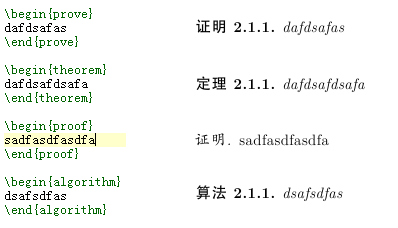
\includegraphics[scale=1]{figures/proofandprove}}
  \figcaption{proof、prove以及部分其他数学环境的差异}
  \label{pic:proofandprove}
\end{figure}

\section{使用模板的一些建议}

公式、章节、图和表格等(不包括脚注和参考文献)的交叉引用可以使用\verb|\autoref{label}|来得到正确的引用。例如使用\verb|\autoref{some_pic}|可以得到“图 X”的引用,使用\verb|\autoref{some_table}|可以得到“表 X”的引用。

建议使用\verb|\figcaption{}|命令得到所有图形的标题,表格也是。这样无论是否在图形环境中均能够得到正确的带图/表编号的标题,而在图形环境之外使用\verb|\caption{}|命令会报错。

%封面是按照制本厂的要求制作的,其中行宽和行高都是固定的,中文标题最多占两行,英文标题最多占三行。如果您的题目超过了这个限制,请缩减题目长度,不要擅自修改模板中的相关配置参数。

